\documentclass[11pt,a4paper]{article}

\usepackage[T1]{fontenc}
\usepackage[utf8]{inputenc}
\usepackage{amsmath,amssymb}
\usepackage{graphicx}
\usepackage{booktabs}
\usepackage{enumitem}
\usepackage{listings}
\usepackage{placeins}
\renewcommand{\thetable}{S\arabic{table}}
\renewcommand{\thefigure}{S\arabic{figure}}
\AtBeginDocument{\renewcommand{\thelstlisting}{S\arabic{lstlisting}}}
\usepackage[colorlinks=true,linkcolor=blue,urlcolor=blue]{hyperref}
\usepackage{geometry}
\geometry{margin=1in}
\setlength{\emergencystretch}{3em}

% Model, detector, and context names used in the paper.
\newcommand{\proprietaryLLM}{gpt-5-mini-2025-08-07}
\newcommand{\openSourceLLMOne}{Llama-3.1-70B-Instruct}
\newcommand{\openSourceLLMTwo}{Qwen2.5-72B-Instruct}
\newcommand{\zeroGptDetector}{ZeroGPT}
\newcommand{\robertaDetector}{ChatGPT Detector RoBERTa}
\newcommand{\robertaQaDetector}{ChatGPT-QA Detector RoBERTa}
\newcommand{\binocularsDetector}{Binoculars}
\newcommand{\FileCont}{Full Code}
\newcommand{\LinkedIssues}{Linked Issue}
\newcommand{\WithoutFileContents}{Multi-source}

\title{\textbf{Supplementary Material}\\[0.5em]
\large\textit{Context, Semantics, and Alignment in AI-Generated Pull Request Descriptions}}
\author{Ayobami Joshua Joseph, Youmei Fan, Sebastian Baltes, Christoph Treude,\\
Kenichi Matsumoto, Raula Gaikovina Kula}
\date{}

\begin{document}
\maketitle

This document reports supplementary methods and results for the paper
\textit{``Context, Semantics, and Alignment in AI-Generated Pull Request Descriptions.''}
The full replication package, including datasets, analysis notebooks, and code, is available
in the \href{https://github.com/NAIST-SE/generated-ai-pull-requests-replication}{public
GitHub repository}.

It documents sampling and reference-audit details and provides additional descriptive detail for the Preliminary Question and post-hoc
\binocularsDetector~robustness check, RQ2 structural and lexical distributions,
ROUGE, BERTScore, and fixed-corpus BM25 retrieval results,
and an example generation prompt. Tables, figures, and listings use an S prefix to
distinguish them from those in the main paper.

\section{Sampling and Reference Audit}
\label{sec:sampling_reference_audit}

We selected a simple random sample of 308 PRs from the filtered population of 1,536 PRs. Sample size was set using the finite-population formula for a binary proportion with 95\% confidence, a 5\% margin of error, and $p=0.5$. These assumptions set the sample size, not a power or precision guarantee for the subsequent metrics. The sampled distributions of word count, total churn, and changed-file count visually track the same distributions in the filtered population. We treat this agreement as a descriptive check rather than proof of representativeness.

For each sampled PR, we collected patch-level, file-level, and referenced-artifact data through the GitHub REST API. A post-collection audit traced every reference back to its PR body and verified the corresponding API object type. The sample contains 352 PR--artifact references representing 343 unique artifacts: 293 references to 284 genuine issues and 59 references to pull requests. Of the 308 sampled PRs, 273 reference at least one genuine issue and 35 reference pull requests only. We retained all 308 PRs for the human baseline and the Repo Path, PR Title, Patch, and Full Code configurations; Linked Issue and Multi-source were restricted to the 273 genuine-issue PRs. Manual review also confirmed that the retained issues fall within the same study time window as their corresponding PRs. The resulting dataset contains 2,523 diff hunks and 1,344 modified files.

\section{Preliminary Question}

The corrected run of the three pre-specified detectors scores every description and produces no false positives on the 308
human baselines in the Patch comparison, so specificity is 1.000 in every cell. Detection
sensitivity is nevertheless strongly model dependent. For \proprietaryLLM,
\robertaDetector~has recall 0.006 (F1 0.013), \robertaQaDetector~flags no descriptions, and
\zeroGptDetector~has recall 0.143 (F1 0.250). For \openSourceLLMOne, the corresponding F1
scores are 0.235, 0.156, and 0.000. The strongest baseline signal occurs for
\openSourceLLMTwo: F1 is 0.335 for \robertaDetector, 0.698 for \robertaQaDetector, and 0.606
for \zeroGptDetector.

On paired binary decisions for the same 308 PRs, flag rates differ across generators for every
detector: \zeroGptDetector~($Q(2)=177.2$), \robertaDetector~($Q(2)=61.8$), and
\robertaQaDetector~($Q(2)=277.8$), all $p<0.001$. All nine exact McNemar comparisons remain
significant after one Benjamini--Hochberg correction; eight have $p_{adj}<0.001$, while the
\robertaDetector~comparison between the two open-source models has $p_{adj}=0.019$.

\section{Detection Performance Uncertainty}

Table~\ref{tab:human_false_positive_intervals} reports human false-positive rates;
Table~\ref{tab:pooled_recall_intervals} reports recall pooled over available contexts;
Tables~\ref{tab:context_recall_intervals_1}--\ref{tab:context_recall_intervals_3} report
recall for every detector--model--context combination.
Cell-level recall and human false-positive rates use two-sided 95\% Wilson intervals.
Pooled recall retains the verified 2,000-replicate PR-clustered percentile-bootstrap
intervals, preserving dependence between descriptions of the same PR. The human baseline
contains 308 unique descriptions and is reused across comparisons, not multiplied by
the number of models or contexts. Intervals are pointwise, not simultaneous; they do not
measure variation across projects or repeated generations. All thresholds and observed
decisions are unchanged.

% Generated; pointwise intervals, not simultaneous comparisons.
\begin{table}[htbp]
\centering
\caption{Human false-positive rates on the 308 unique human descriptions. Intervals are 95\% Wilson intervals; these baselines are reused, not independent samples for each model or context.}
\label{tab:human_false_positive_intervals}
\small
\setlength{\tabcolsep}{4pt}
\renewcommand{\arraystretch}{1.15}
\begin{tabular}{lrrr}
\toprule
\textbf{Detector} & \textbf{False positives} & \textbf{Human $n$} & \textbf{FPR (\%) [95\% CI]} \\
\midrule
RoBERTa & 0 & 308 & 0.0 [0.0, 1.2] \\
RoBERTa-QA & 0 & 308 & 0.0 [0.0, 1.2] \\
ZeroGPT & 0 & 308 & 0.0 [0.0, 1.2] \\
Binoculars & 4 & 308 & 1.3 [0.5, 3.3] \\
\bottomrule
\end{tabular}
\end{table}

\begin{table}[htbp]
\centering
\caption{Recall (\%) pooled over available contexts, with the existing 95\% PR-clustered percentile-bootstrap intervals (2,000 replicates). AI counts are 1,772 for Qwen and GPT, 1,778 for Llama, and 5,322 overall. Binoculars is post-hoc.}
\label{tab:pooled_recall_intervals}
\small
\setlength{\tabcolsep}{4pt}
\renewcommand{\arraystretch}{1.15}
\begin{tabular}{lrrrr}
\toprule
\textbf{Detector} & \textbf{Qwen2.5-72B} & \textbf{GPT-5-mini} & \textbf{Llama-3.1-70B} & \textbf{All models} \\
\midrule
RoBERTa & 35.8 [33.2, 38.3] & 0.4 [0.1, 0.7] & 28.7 [26.6, 31.0] & 21.6 [20.3, 23.0] \\
RoBERTa-QA & 63.7 [61.1, 66.3] & 0.1 [0.0, 0.2] & 17.5 [15.6, 19.4] & 27.1 [25.9, 28.3] \\
ZeroGPT & 46.5 [44.0, 49.1] & 20.6 [18.7, 22.6] & 1.9 [1.2, 2.5] & 23.0 [21.7, 24.2] \\
Binoculars & 59.7 [57.3, 62.2] & 1.5 [1.0, 2.1] & 25.9 [23.8, 28.1] & 29.0 [27.8, 30.3] \\
\bottomrule
\end{tabular}
\end{table}
\FloatBarrier

\begin{table}[htbp]
\centering
\caption{Recall (\%) by context for Qwen2.5-72B, with 95\% Wilson intervals. Each column retains the detector's recorded decision rule; Binoculars is post-hoc.}
\label{tab:context_recall_intervals_1}
\small
\setlength{\tabcolsep}{4pt}
\renewcommand{\arraystretch}{1.15}
\begin{tabular}{lrrrrr}
\toprule
\textbf{Context} & \textbf{AI $n$} & \textbf{RoBERTa} & \textbf{RoBERTa-QA} & \textbf{ZeroGPT} & \textbf{Binoculars} \\
\midrule
Repo Path & 308 & 23.7 [19.3, 28.8] & 40.6 [35.2, 46.2] & 49.0 [43.5, 54.6] & 33.1 [28.1, 38.6] \\
PR Title & 308 & 69.8 [64.5, 74.7] & 78.6 [73.7, 82.8] & 21.4 [17.2, 26.3] & 70.5 [65.1, 75.3] \\
Patch & 308 & 20.1 [16.0, 25.0] & 53.6 [48.0, 59.1] & 43.5 [38.1, 49.1] & 64.3 [58.8, 69.4] \\
Full Code & 302 & 36.8 [31.5, 42.3] & 81.8 [77.0, 85.7] & 68.2 [62.8, 73.2] & 68.9 [63.4, 73.8] \\
Linked Issue & 273 & 41.8 [36.1, 47.7] & 63.7 [57.9, 69.2] & 44.3 [38.5, 50.3] & 54.2 [48.3, 60.0] \\
Multi-source & 273 & 21.6 [17.1, 26.9] & 64.5 [58.6, 69.9] & 53.5 [47.6, 59.3] & 67.8 [62.0, 73.0] \\
\bottomrule
\end{tabular}
\end{table}

\begin{table}[htbp]
\centering
\caption{Recall (\%) by context for GPT-5-mini, with 95\% Wilson intervals. Each column retains the detector's recorded decision rule; Binoculars is post-hoc.}
\label{tab:context_recall_intervals_2}
\small
\setlength{\tabcolsep}{4pt}
\renewcommand{\arraystretch}{1.15}
\begin{tabular}{lrrrrr}
\toprule
\textbf{Context} & \textbf{AI $n$} & \textbf{RoBERTa} & \textbf{RoBERTa-QA} & \textbf{ZeroGPT} & \textbf{Binoculars} \\
\midrule
Repo Path & 308 & 0.0 [0.0, 1.2] & 0.0 [0.0, 1.2] & 30.2 [25.3, 35.5] & 1.6 [0.7, 3.7] \\
PR Title & 308 & 0.6 [0.2, 2.3] & 0.3 [0.1, 1.8] & 32.1 [27.2, 37.6] & 4.9 [3.0, 7.9] \\
Patch & 308 & 0.6 [0.2, 2.3] & 0.0 [0.0, 1.2] & 14.3 [10.8, 18.6] & 0.0 [0.0, 1.2] \\
Full Code & 302 & 0.3 [0.1, 1.9] & 0.0 [0.0, 1.3] & 3.6 [2.0, 6.4] & 0.0 [0.0, 1.3] \\
Linked Issue & 273 & 0.0 [0.0, 1.4] & 0.0 [0.0, 1.4] & 28.2 [23.2, 33.8] & 1.8 [0.8, 4.2] \\
Multi-source & 273 & 0.7 [0.2, 2.6] & 0.0 [0.0, 1.4] & 15.0 [11.3, 19.7] & 0.7 [0.2, 2.6] \\
\bottomrule
\end{tabular}
\end{table}

\begin{table}[htbp]
\centering
\caption{Recall (\%) by context for Llama-3.1-70B, with 95\% Wilson intervals. Each column retains the detector's recorded decision rule; Binoculars is post-hoc.}
\label{tab:context_recall_intervals_3}
\small
\setlength{\tabcolsep}{4pt}
\renewcommand{\arraystretch}{1.15}
\begin{tabular}{lrrrrr}
\toprule
\textbf{Context} & \textbf{AI $n$} & \textbf{RoBERTa} & \textbf{RoBERTa-QA} & \textbf{ZeroGPT} & \textbf{Binoculars} \\
\midrule
Repo Path & 308 & 23.4 [19.0, 28.4] & 11.0 [8.0, 15.0] & 0.6 [0.2, 2.3] & 8.8 [6.1, 12.5] \\
PR Title & 308 & 58.4 [52.9, 63.8] & 24.7 [20.2, 29.8] & 0.6 [0.2, 2.3] & 45.1 [39.7, 50.7] \\
Patch & 308 & 13.3 [10.0, 17.6] & 8.4 [5.8, 12.1] & 0.0 [0.0, 1.2] & 16.6 [12.8, 21.1] \\
Full Code & 308 & 38.0 [32.7, 43.5] & 26.0 [21.4, 31.1] & 5.8 [3.7, 9.0] & 35.1 [29.9, 40.5] \\
Linked Issue & 273 & 15.8 [11.9, 20.5] & 12.5 [9.1, 16.9] & 1.5 [0.6, 3.7] & 16.1 [12.2, 20.9] \\
Multi-source & 273 & 21.2 [16.8, 26.5] & 22.7 [18.1, 28.0] & 2.6 [1.2, 5.2] & 33.7 [28.4, 39.5] \\
\bottomrule
\end{tabular}
\end{table}

\FloatBarrier


\section{Post-hoc Binoculars Robustness Check}

After the pre-specified three-detector analysis, we scored the same 5,630 descriptions with
\binocularsDetector, a zero-shot detector based on an official Falcon-7B/Falcon-7B-Instruct
pair. We retained the authors' low-false-positive-rate threshold, BF16 precision, and 512-token
limit; no threshold was tuned on the study corpus. The source and model revisions were pinned.
A reviewed Apple-MPS fork changed device and memory handling but not the scoring formula,
model pair, threshold, or input text. Two repetitions of ten frozen smoke records exactly
reproduced the submitted scores. Fast-DetectGPT was not run and is not part of this analysis.

\begin{table}[htbp]
\centering
\caption{Post-hoc \binocularsDetector~performance across pooled contexts. Intervals are 95\%
percentile intervals from 2,000 PR-clustered bootstrap replicates. The same 308 human
descriptions are used in every generator row.}
\label{tab:binoculars_pooled}
\small
\setlength{\tabcolsep}{4pt}
\begin{tabular}{lrrrr}
\toprule
\textbf{Generator} & \textbf{AI $n$} & \textbf{Recall [95\% CI]} & \textbf{F1 [95\% CI]} & \textbf{AUROC [95\% CI]} \\ \midrule
Qwen2.5-72B & 1,772 & 0.597 [0.573, 0.622] & 0.747 [0.727, 0.766] & 0.942 [0.927, 0.955] \\
gpt-5-mini & 1,772 & 0.015 [0.010, 0.021] & 0.030 [0.020, 0.041] & 0.637 [0.606, 0.668] \\
Llama-3.1-70B & 1,778 & 0.259 [0.238, 0.281] & 0.411 [0.384, 0.438] & 0.634 [0.609, 0.658] \\ \midrule
Pooled & 5,322 & 0.290 [0.278, 0.303] & 0.450 [0.435, 0.465] & 0.737 [0.717, 0.756] \\ \bottomrule
\end{tabular}
\end{table}

\binocularsDetector~flags four of 308 human descriptions, giving a false-positive rate of
0.013 (95\% Wilson CI [0.005, 0.033]) and specificity 0.987; the three pre-specified
detectors flag none, with false-positive-rate intervals [0.000, 0.012]. On the same 5,322 AI descriptions,
its pooled recall exceeds \zeroGptDetector, \robertaDetector, and \robertaQaDetector~by 0.061
(95\% CI [0.046, 0.077]), 0.074 [0.058, 0.090], and 0.020 [0.003, 0.037], respectively.
However, the pooled AUROC in Table~\ref{tab:binoculars_pooled} is below those of both RoBERTa
detectors (0.864 and 0.885). The threshold comparison therefore does not establish uniformly
stronger discrimination.

On per-PR scores averaged across the available generators, the six context ranks differ
($\chi^2(5)=267.0$, $n=273$, $p<0.001$). Fourteen of the 15 paired Wilcoxon contrasts remain
significant after a separate Benjamini--Hochberg correction; only Patch versus Linked Issue
is non-significant ($p_{adj}=0.669$, $r_{rb}=-0.030$). PR Title has the highest pooled median AI
score and Repo Path the lowest. Model-specific F1 ranges are 0.493--0.820 for Qwen,
0.159--0.616 for Llama, and 0.000--0.092 for gpt-5-mini. These post-hoc results corroborate
generator and context sensitivity rather than supplying a universal context ordering.

All 5,630 \binocularsDetector~calls succeeded; 268 inputs (4.76\%) were truncated at 512 tokens.
The public replication package provides the exact analysis source, the unchanged 22,520-row
record-level score table, aggregate tables, independent verification, and sanitized
source/model/environment provenance. Detector scores and predicted labels are experimental
measurements, not evidence of the authorship of any real pull request. The relevant package list is
not represented as a complete transitive lock, and the complete run was not independently
repeated on CUDA. The results therefore remain tied to the recorded model revisions, global
threshold, and Apple-MPS implementation.

\section{RQ2: Textual Similarity}

\subsection{Structural and lexical metric distributions}

Figures~\ref{fig:fkgl_boxplots}--\ref{fig:ld_boxplots} present the per-context distributions
for FKGL, TTR, bidirectional MTLD, and lexical density, complementing
the matched readability/lexical median/quartile table and paired effect-size tables retained in the main paper.
Each figure
compares the distribution of AI-generated descriptions with the human baseline across the
six context configurations.

\begin{figure}[htbp]
    \centering
    \includegraphics[page=2,width=\textwidth]{figures/textual_features_boxplots.pdf}
    \caption{Readability (FKGL) distributions (RQ2).}
    \label{fig:fkgl_boxplots}
\end{figure}

\begin{figure}[htbp]
    \centering
    \includegraphics[page=3,width=\textwidth]{figures/textual_features_boxplots.pdf}
    \caption{Type--Token Ratio (TTR) distributions (RQ2).}
    \label{fig:ttr_boxplots}
\end{figure}

\begin{figure}[htbp]
    \centering
    \includegraphics[page=4,width=\textwidth]{figures/textual_features_boxplots.pdf}
    \caption{Measure of Textual Lexical Diversity (MTLD) distributions (RQ2).}
    \label{fig:mtld_boxplots}
\end{figure}

\begin{figure}[htbp]
    \centering
    \includegraphics[page=5,width=\textwidth]{figures/textual_features_boxplots.pdf}
    \caption{Lexical Density (LD) distributions (RQ2).}
    \label{fig:ld_boxplots}
\end{figure}

\subsection{Similarity metrics}

\begin{enumerate}[leftmargin=*,noitemsep,topsep=2pt,parsep=0pt]
    \item \textbf{ROUGE}: Figure~\ref{fig:rouge_boxplots} reports direct
    generated-to-reference lexical overlap. \WithoutFileContents~has the highest median overlap
    for all three models, whereas \LinkedIssues~alone does not. Even in the top-ranked context,
    unigram overlap is moderate and
    bigram overlap remains low. The lowest-ranked configuration varies, so these results do
    not support a universal raw-code or minimal-context ordering. We do not test against a
    human self-comparison baseline, because a description compared with itself produces a
    degenerate score rather than an empirical human distribution.

    \item \textbf{BERTScore}: Figure~\ref{fig:bertscore_boxplots} shows that
    \WithoutFileContents~has the highest generated-to-reference BERTScore median for all three
    models, with a maximum baseline-rescaled median F1 of 0.003 for \proprietaryLLM. Because
    baseline rescaling was enabled, these
    scores may be negative and should not be interpreted as percentages. The result
    establishes a relative ordering among the evaluated configurations, not that ``why''
    metadata is inherently more effective than ``what'' metadata. Lower scores for some
    \FileCont~cells may partly reflect truncation, particularly for \proprietaryLLM. As with
    ROUGE, we do not use the degenerate human self-comparison as an inferential baseline.

    \item \textbf{BM25 retrieval}: Figure~\ref{fig:bm25_retrieval} reports reciprocal rank
    against one fixed corpus of all 308 human descriptions, avoiding the retired per-cell
    normalisation and degenerate human self-score. \WithoutFileContents~has the highest MRR for
    every model: 0.509 for \openSourceLLMTwo, 0.527 for \proprietaryLLM, and 0.554 for
    \openSourceLLMOne. It retrieves the paired human description at rank 1 for 45.1\%, 46.5\%,
    and 50.9\% of their respective queries. Context ranks differ for every model (Friedman
    $\chi^2(5)=291.5$, 254.9, and 263.3; $n=267$, 267, and 273, respectively; all
    $p<0.001$). All 15 pre-specified Linked-Issue-versus-other-context contrasts remain
    significant after one FDR correction ($p_{adj}\leq0.0034$), but their directions are mixed.
\end{enumerate}

\begin{figure}[htbp]
    \centering
    \includegraphics[page=6,width=\textwidth]{figures/textual_features_boxplots.pdf}
    \caption{Lexical overlap (ROUGE-L F1) distributions (RQ2).}
    \label{fig:rouge_boxplots}
\end{figure}

\begin{figure}[htbp]
    \centering
    \includegraphics[page=7,width=\textwidth]{figures/textual_features_boxplots.pdf}
    \caption{BERTScore F1 distributions against the paired human description, with baseline
    rescaling enabled (RQ2).}
    \label{fig:bertscore_boxplots}
\end{figure}

\begin{figure}[htbp]
    \centering
    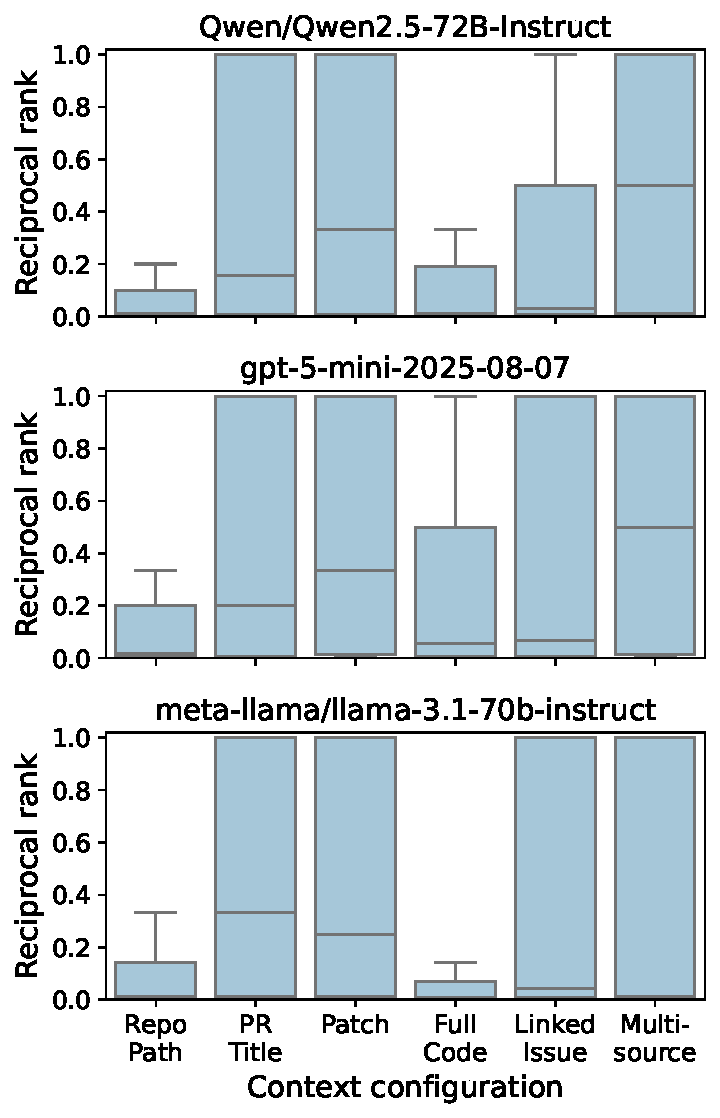
\includegraphics[width=0.65\textwidth]{figures/bm25_retrieval_portrait.pdf}
    \caption{Fixed-corpus BM25 reciprocal-rank distributions (RQ2). Each AI description
    queries the corpus of 308 human descriptions; the human description for the same PR is
    the sole relevant document. Higher values indicate that the paired human description
    was retrieved nearer the top.}
    \label{fig:bm25_retrieval}
\end{figure}

Across the structural and lexical measures, differences from the paired human descriptions
depend on the model, metric, and configuration; neither minimal, code-dense, nor narrative
configurations are uniformly closest to the human baseline. The ROUGE and BERTScore results
show that generated-to-reference similarity varies by configuration, with Multi-source
obtaining the highest medians for all three models. The fixed-corpus BM25 analysis likewise
ranks Multi-source highest by MRR for all three models. Linked Issue alone is not the
top configuration. These measures do not define a
percentage of human similarity, and they do not establish factual correctness or review
adequacy.

\FloatBarrier

BERTScore's 512-token limit truncated the AI side of 4.85\% of the 5,322 corrected pairs. When
either the AI or paired human description is considered, 9.88\% of pairs were affected, with
64,066 input tokens removed (2.94\% of all input tokens). AI-side truncation was highest for
\proprietaryLLM~under \FileCont~(23.51\%), so that cell should be interpreted cautiously.
\section{Example Generation Prompt}

Supplementary Listing~\ref{lst:sample_prompt} preserves the example Repo Path prompt
from the main paper. The same base instruction and JSON output format were used
across all six configurations; only the supplied context block varied. The full
set of templates is retained in the replication package. The file paths below are
example input, not an additional experimental condition.

% Relocated from Overleaf be05c0b; the prompt body is unchanged.
\begin{lstlisting}[
    basicstyle=\ttfamily\footnotesize,
    frame=single,
    breaklines=true,
    caption={Prompt for the Repo Path context configuration.},
    label={lst:sample_prompt},
    captionpos=b,
    morekeywords={CONTEXT, END, JSON}
]
"You are a helpful assistant that generates GitHub pull request
descriptions. Based on the provided context, write a clear and
informative description. Respond with ONLY a JSON object in this
format: {"description": "<your description here>"}
Do not include any other text or explanation.

### CONTEXT
<repository>JabRef/jabref</repository>

<affected_files>
CHANGELOG.md
src/main/java/org/jabref/JabRefMain.java
</affected_files>
### END CONTEXT

Reminder: based on the provided context, write a clear and
informative description. Respond with ONLY a JSON object in
this format: {"description": "..."}.
\end{lstlisting}


\end{document}
